\section{Feature Extraction}
In order to correctly extract features from the cleaned data, we had to consider a couple of different feature extraction techniques, such as, Term Frequency, Term Frequency-Inverse Document Frequency and Sentiment Analysis.

\subsection{Term Frequency}

When classifying text files a logical first feature to take a look at is Term-Frequency (TF).
TF just counts for each token the number of time it appears in the text file.
However, there are different ways to approach this. 
Instead of using a single word as a token it is possible to take any number of words that appear sequentially  as a feature, this is called an n-gram.

\subsection{Term Frequency- Inverse Document Frequency}

A way to counter the problems TF has we can use Term Frequency-Inverse Document Frequency (TF-IDF).
Instead of just looking at how frequently a term is in the document we also look at how common it is across all documents.
In that way, common terms across all documents become less important features, while terms that are special to a document become more important.

We explored for TF-IDF at different ranges of \textit{n-gram} options to determine what gave the best results, see Figure~\ref{fig:ngram}.
Interestingly a \textbf{unigram} (1-gram) gave the best results when using an out-of-the-box logistic regressor. So we stuck with that for our advanced models but also did an analysis of the model's performance using different n-gram ranges.

 \begin{figure*}[ht!]
    \centering
    \subfloat[F1-score for different n-gram ranges\label{fig:ngram-f1}]{%
        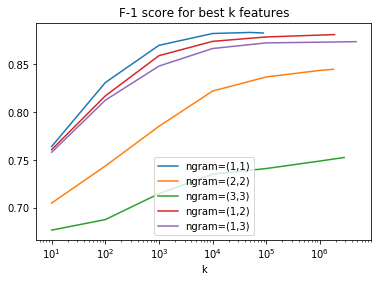
\includegraphics[width=0.3\linewidth]{figures/ngram_range/f1-score.png}}
    \hfill
    \subfloat[Precision-score for different n-gram ranges\label{fig:ngram-precision}]{%
        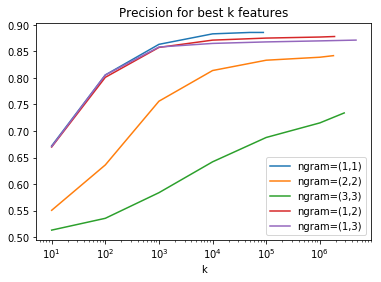
\includegraphics[width=0.3\linewidth]{figures/ngram_range/precision-score.png}}
        \hfill
    \subfloat[Recall-score for different n-gram ranges\label{fig:ngram-recall}]{%
        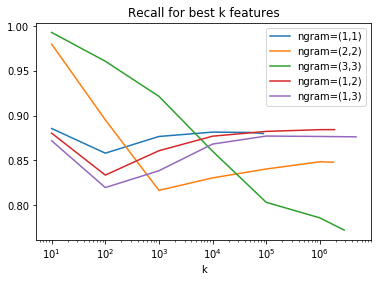
\includegraphics[width=0.3\linewidth]{figures/ngram_range/recall-score.png}}
  \caption{Scores for different N-gram ranges.}
  \label{fig:ngram} 
\end{figure*}

\subsection{Sentiment Analysis}
The previous two features TF and TF-IDF are focusing on frequency of the words that appear in a document, but it doesn't make any distinction between the words.
The third feature we are looking at focusing exactly on this problem. Instead of looking at individual words, we can look at each review on its own and determine its sentiment.
Achieving this is done by applying \textit{Valence Aware Dictionary and Sentiment Reasoner}, also known as VADER, on each review.
For each review we then get a tuple with four values: positive, compound, neutral, or negative. The first value is a summarized score These features can then be used to train a classifier. 

\subsection{Bag of Words Model and Word2Vec for RNN Analysis}
Bag of Words is a representation of words(text) in natural language processing where we pick top "W" words among all the reviews and search for most words among the "W" words that exists within the reviews where each review is represented as N-dimensional feature vector. The positioning of these words do not matter, rather just the frequency. The reason we need to pick top "W" words out of all the unique words is to reduce the dimension of the data points. Although this is the most basic model, preprocessing is applied beforehand to remove the unimportant words and clean the text. While BoW is good to classify documents as a whole, Word2Vec is great for identifying the content within the data present. Word2Vec produces the one vector per word hence the dimension comes out to be very large to search the whole corpus within.  


\subsection{Comparison}

When the three different set of features are compared, Table-\ref{tab:features-comp}, we can see clearly that TF-IDF is performing best out of the three, closely followed by TF, and on a distance Sentiment analysis using VADER.
It is interesting that VADER, did not perform better. It shows that it is very complex to summarize a text down to just four values.
It still performs considerably better than random, but there is a big gap in performance between TF-IDF and VADER. So we decided to stick with TF-IDF for our advanced models.

\begin{table}[ht!]
    \centering
    \caption{Results for different features using an out-of-the-box Logistic Regressor\label{tab:features-comp}}
    \begin{tabular}{ l| S[table-format=1.3] |S[table-format=1.3] |S[table-format=1.3] }
    \hline
        \bf{Feature} & \bf{F1-measure} & \bf{Precision} & \bf{Recall} \\
    \hline
        TF & 0.868 & 0.876 & 0.859 \\ 
        TF-IDF & 0.886 & 0.883 & 0.889 \\
        VADER & 0.719 & 0.716 & 0.721 \\
        \hline
    \end{tabular}
\end{table}

\subsection{Feature Extraction Pipeline}
Based on the results that we found for each feature, we present our feature extraction pipeline in Figure~\ref{fig:feature-selection}.
We chose to use TF-IDF over TF and VADER because of the clearly better performance it gives.
For n-gram-range we chose a range of (1,1), meaning we will only use unigrams.
Unigrams seemed to give the best performance as can be seen in Figure~\ref{fig:ngram}.

\begin{figure}[ht!]
    \setlength{\unitlength}{0.14in}
    \centering
    \begin{picture}(20,10)
    \put(2,4){\framebox(5,3){\footnotesize{TF}}}
    \put(8,4){\framebox(5,3){\footnotesize{TF-IDF}}}
    \put(14,4){\framebox(5,3){\footnotesize{KBest}}}
    \put(1,1.5){\framebox(19,8){}}
    
    \put(0,5.5){\vector(1,0){2}}
    \put(7,5.5){\vector(1,0){1}}
    \put(19,5.5){\vector(1,0){2}}
    
    \end{picture}
    \caption{Pipeline for the Feature Selection}
    \label{fig:feature-selection}
\end{figure}
